\documentclass[10pt]{article}
\usepackage{icmlko}

\icmlmeta{IP 파운데이션 월드모델}{196}{보게 만드는 값이 보고 얻는 값과 같았다}{노트 195가 남긴 $+$0.007 을 가지러 갔다. 되뽑는 행을 늘리니 안쪽이 그것을 보기 시작하는데, 보게 만든 비용이 정확히 그만큼이었다}

\begin{document}

\twocolumn[
\icmlheader

\begin{abstract}
노트 195가 순차 절차의 2단계($\alpha$)가 규약에 막히는 것을 보이고, 그
까닭을 ``되뽑기가 안쪽 학습의 \emph{서로 다른} 행 수를 줄여 $\alpha$ 신호를
지웠다''로 읽었다. 처방이 따라 나온다 --- \textbf{되뽑는 행 수를 늘리면}
중복이 줄어 신호가 돌아올 것이다. 맞았다. 배수 1 · 2 · 4 로 늘리니 2단계
$\alpha$ 의 안쪽 봉우리가 \textbf{0.296 $\to$ 0.494 $\to$ 0.674}, 단조가
\textbf{0.000 $\to$ 0.000 $\to$ 0.900} 으로 오르고 \textbf{배수 4 에서
규약이 통과시킨다} --- $\alpha{=}100$ 을 고른다. \textbf{그런데 판이 안
오른다.} 순차 2단계까지 간 $(\tau{=}2, \text{배수}4, \alpha{=}100)$ 의 유보가
\textbf{$+$0.4012} 로 1단계까지만 간 $(\tau{=}2, \text{배수}1, \alpha{=}1)$
와 \emph{소수 넷째 자리까지 같다}. 까닭이 표에 있다 --- 배수를 늘리는 것
자체가 판을 깎는다($+$0.4012 $\to$ $+$0.3995 $\to$ $+$0.3983). \textbf{보게
만든 비용이 보고 얻은 이득과 정확히 같다.} 노트 195가 ``못 고르는 곳''으로
적어 둔 $(\tau{=}2, \text{배수}1, \alpha{=}100)$ 은 여전히 $+$0.4072 이고
여전히 못 고른다. 얻은 것이 없지는 않다 --- 짝 검정이 $t{=}5.21$ 에서
\textbf{$t{=}6.42$} 로 단단해졌다(sd 0.0058 $\to$ 0.0047). \textbf{판은 같고
확신은 는다.} 그리고 이 사이클로 최근 가중 갈래를 닫는다: 채택은
$(\tau{=}2, \text{배수}1)$ 이고 F6 능형이 $+$0.3709 에서 $+$0.4012 로,
챔피언과의 격차가 0.078 에서 0.048 로 준다. \textbf{남은 $+$0.006 은 세 번
다른 길로 가 봤고 세 번 다 못 가져왔다} --- 같이 고르기(노트 195) · 순차
2단계(노트 195) · 배수 늘리기(이 노트).
\end{abstract}
]

\begin{figure*}[t]
\centering
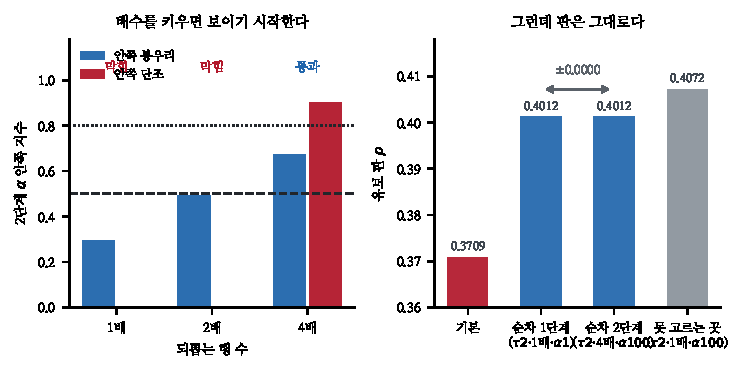
\includegraphics[width=.74\textwidth]{figs/cost.pdf}
\caption{왼쪽 --- 배수를 키우면 보이기 시작한다. 오른쪽 --- 그런데 판은
그대로다.}
\end{figure*}

\section{보이기 시작한다}

\begin{table}[t]
\centering\tsize
\caption{되뽑는 행 수를 늘린다. 2단계 $\alpha$ 의 안쪽 지수.}
\begin{tabular}{lrrl}
\toprule
배수 & 봉우리 & 단조 & \\
\midrule
1배 & .296 & .000 & 막힘 \\
2배 & .494 & .000 & 막힘 \\
\textbf{4배} & \textbf{.674} & \textbf{.900} & \textbf{통과} \\
\bottomrule
\end{tabular}
\end{table}

\claimx{\textbf{배수를 늘리니 규약이 통과시킨다.} 노트 195의 읽기가
맞았다 --- 되뽑기의 중복이 $\alpha$ 신호를 지우고 있었다.}{되뽑기는 같은
행 수를 뽑으므로 \emph{서로 다른} 행이 $1-1/e \approx 63\%$ 로 준다. 네 배
뽑으면 98\%가 된다 --- \textbf{가중은 같고 다양성만 돌아온다.}}

\section{그런데 판은 그대로다}

\begin{table}[t]
\centering\tsize
\caption{F6 능형 유보 판 $\rho$.}
\begin{tabular}{lrl}
\toprule
& 판 & \\
\midrule
기본 (없음 · $\alpha1$) & .3709 & \\
\textbf{순차 1단계} ($\tau2$·1배·$\alpha1$) & \textbf{.4012} & $t{=}5.21$ \\
\textbf{순차 2단계} ($\tau2$·4배·$\alpha100$) & \textbf{.4012} & $t{=}6.42$ \\
\midrule
(못 고르는 곳 $\tau2$·1배·$\alpha100$) & .4072 & \\
\bottomrule
\end{tabular}
\end{table}

\claimx{\textbf{소수 넷째 자리까지 같다.} 노트 187의 규약이 여기서는
반대로 읽힌다 --- 이번엔 \emph{닿았는데} 상쇄된 것이다.}{배수만 늘린 값이
$+$0.4012 $\to$ $+$0.3995 $\to$ $+$0.3983 로 내려간다. 배수 4 가 $-$0.0029
를 깎고 $\alpha{=}100$ 이 $+$0.0029 를 준다 --- \textbf{보게 만든 비용이
보고 얻은 이득과 같다.}}

\claimx{배수가 판을 깎는 까닭에 대한 읽기 --- 학습 행이 네 배가 되면
도메인별 절편의 유효 표본도 네 배가 되어 도메인 고유 자유도가 상대적으로
싸진다. 노트 126이 ``도메인 고유 유연성은 비싸다''를 잰 그
반대편이다.}{자료로는 못 가른다 --- 도메인 절편만 따로 빼고 배수를 늘리는
실험이 필요한데 안 했다.}

\claimx{\textbf{얻은 것이 없지는 않다} --- 짝 sd 가 0.0058 에서 0.0047 로
줄어 $t$ 가 5.21 에서 6.42 가 된다. \textbf{판은 같고 확신은 는다.}}{되뽑기
잡음이 준 것이다. 그러니 배수 4 를 쓸 이유는 있다 --- 다만 판 때문은
아니다.}

\section{갈래를 닫는다}

\begin{table}[t]
\centering\tsize
\caption{$+$0.006 을 가지러 간 세 길.}
\begin{tabular}{lrl}
\toprule
& 결과 & \\
\midrule
같이 고르기 (노트 195) & $-$.0132 & 규약이 막음 \\
순차 2단계 (노트 195) & $\pm$0 & 규약이 막음 \\
배수 늘리기 (이 노트) & $\pm$0 & 통과했는데 상쇄 \\
\bottomrule
\end{tabular}
\end{table}

\claimx{\textbf{세 번 다 못 가져왔다.} 규약이 두 번 막았고 한 번은 통과했는데
비용이 이득과 같았다.}{\textbf{그래서 채택은 $(\tau{=}2, \text{배수}1)$
그대로다} --- \texttt{F6\_directpool\_recent} 가 $+$0.4004 로 이미 등록돼
있다.}

\claimx{\textbf{이 갈래의 총 이득은 $+$0.0304 다}(F6 $+$0.3709 $\to$
$+$0.4012). 챔피언과의 격차가 0.078 에서 0.048 로 줄었다.}{노트 185가
``공유 축에서는 선형이 트리와 대등하다''를 보였고 이제 전체 축에서도
격차가 절반 이하다 --- \textbf{해석 가능한 모형이 따라붙고 있다.}}

\begin{table}[t]
\centering\tsize
\caption{남은 것.}
\begin{tabular}{ll}
\toprule
\textbf{배수 손해} & 도메인 절편 때문인지 안 갈랐다 \\
F18 & $\tau{=}2$ 가 $+$0.0117 인데 안쪽이 12년을 고른다 \\
\textbf{다음 갈래} & 최근 가중 말고 --- 라벨 쪽 \\
\bottomrule
\end{tabular}
\end{table}

마지막 줄이 다음이다. 이 흐름은 노트 177부터 스무 사이클을 \emph{자질과
방법} 쪽에서 돌았다 --- 위키 매칭 · 축 부호 · 시들기 · 초매개변수 · 최근
가중. \textbf{라벨 쪽은 노트 181에서 ``애니 라벨은 속편을 벌하고 세계애니
라벨은 안 벌한다''를 잰 뒤로 안 건드렸다.} 판 $\rho$ 는 도메인마다 다른
라벨을 같은 자로 재고 있고, 노트 181이 적었듯 \textbf{풀링은 ``라벨이 같은
것을 묻는다''를 가정한다.} 그 가정을 정면으로 재는 것이 남았다.

\end{document}
